%%%%%%%%%%%%%%%%%%%%%%%%%%%%%%%%%%%%%%%%%%%%%%%%%%%%%%%%%%%%%%%%%%%%%%
% This layout was adapted from one found at latextemplates.com which
% was adapted from another.
%
% License: CC BY-NC-SA 3.0
% (http://creativecommons.org/licenses/by-nc-sa/3.0/)
%
% Original header:
%
% This is a LaTeX version of the sample laboratory report from
% Virginia Tech's copyrighted 08-09 CHEM 1045/1046 lab manual.
% Reproduction of this one appendix section for academic purposes
% should fall under fair use.
%
%%%%%%%%%%%%%%%%%%%%%%%%%%%%%%%%%%%%%%%%%%%%%%%%%%%%%%%%%%%%%%%%%%%%%%

\documentclass{article}

\usepackage{graphicx} % Lets us use images
\usepackage[acronym]{glossaries} % Lets us use acronyms

\author{Charles Pittman}
\title{ELEC-311\\ Project 1\\ Combinational Circuit Analysis}
\date{September 17, 2013}

\loadglsentries{acronyms} % Actually loads 'acronyms.tex'
\makeglossaries

\begin{document}

\maketitle % Inserts title, author, and date from above

\pagebreak

% Removes indentation from paragraphs: \setlength\parindent{0pt}

% Number the enumerate environment (unordered lists) by letter:
\renewcommand{\labelenumi}{\alph{enumi}.}

\section{Objective}
\label{sec:objective}

% Multiple objectives:
 \begin{description}
 \item[First Objective] \hfill \\
   Analyze a combinational logic circuit and determine its behavior.
 \item[Second Objective] \hfill \\
   Objective 2 text
 \end{description}

\section{Discussion}
\label{sec:procedure}

The circuit being studied is shown in Figure~\ref{fig:circuit}.
Working from right to left, the Boolean equation for the circuit can
be written: $(\overline{S} \cdot I_0 + I_1) \cdot E \cdot (I_0 + S
\cdot I_1)$.  A truth table for this equation is shown in Table~\ref{tab:truth}.


\begin{figure}[h]
  \centering
%  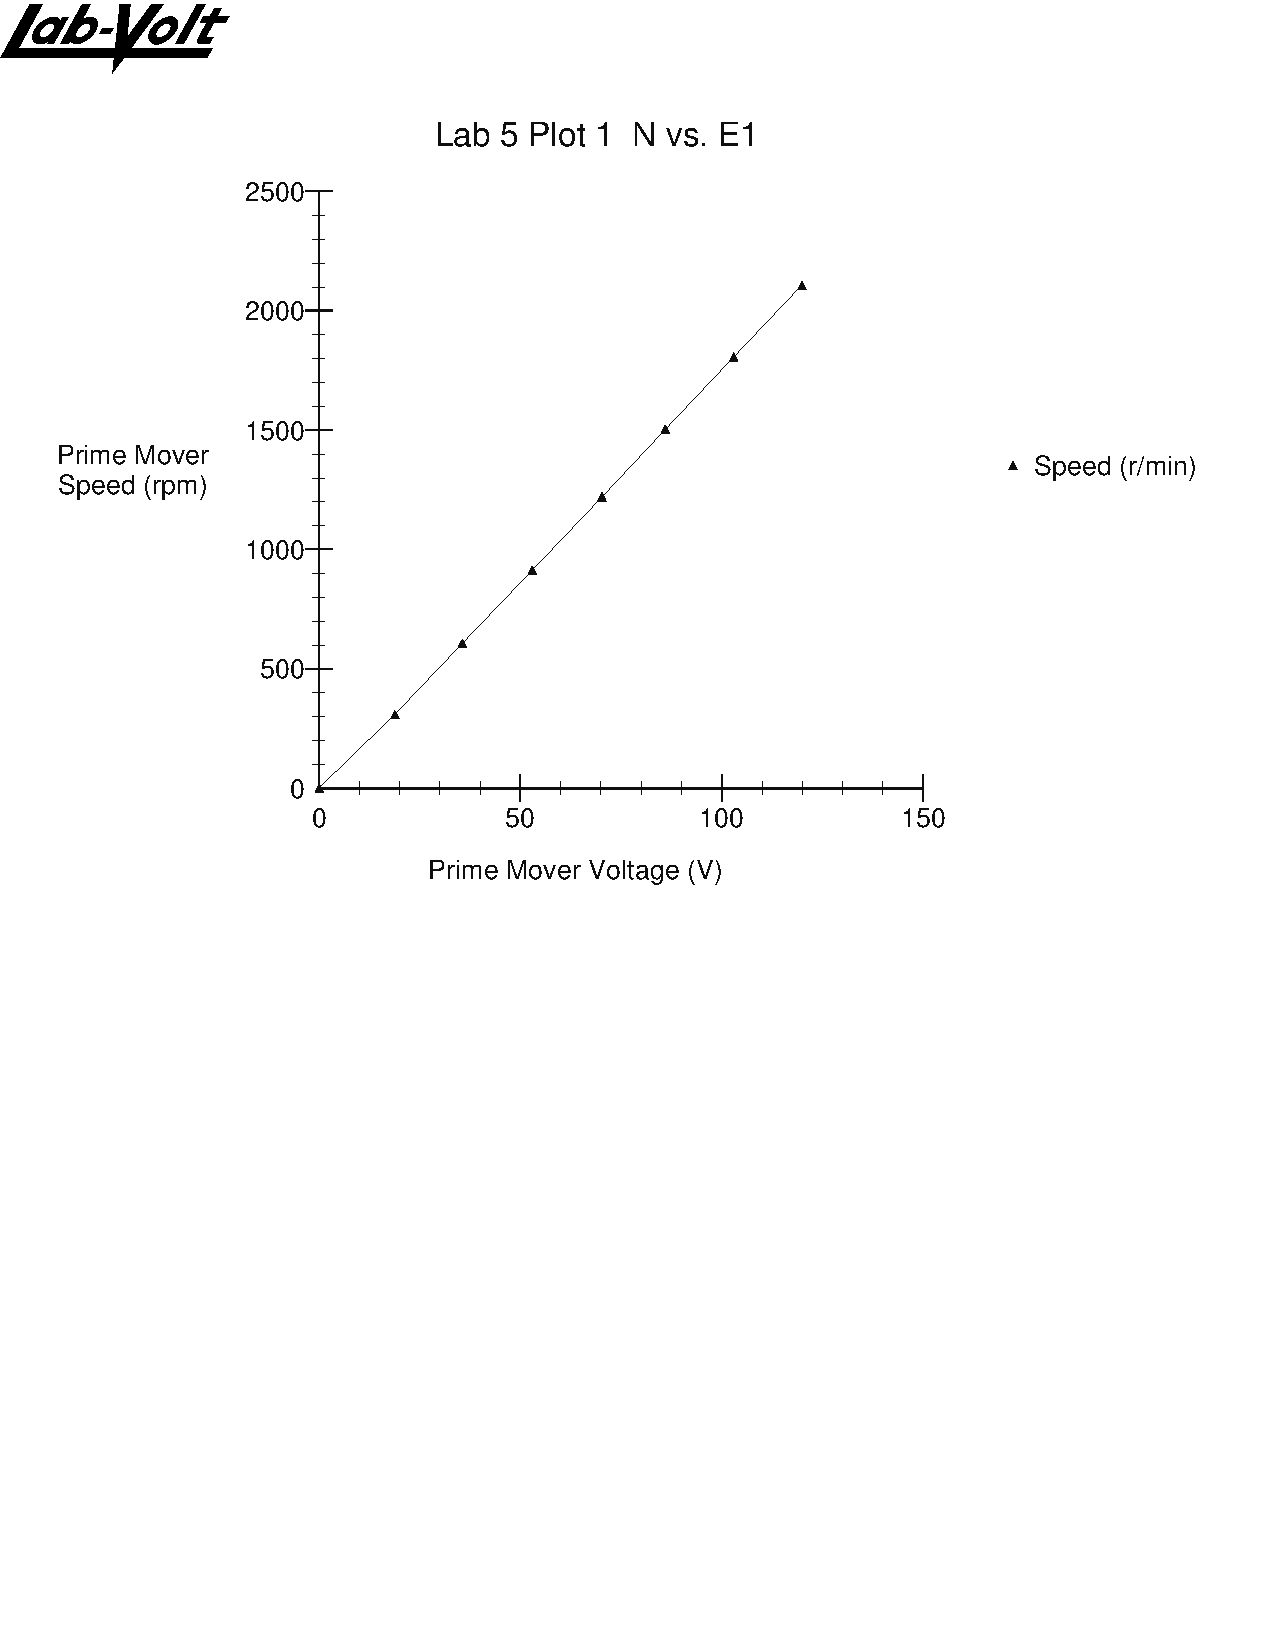
\includegraphics[width=\textwidth]{img/plot1}
  \caption{Circuit to be analyzed.}
  \label{fig:circuit}
\end{figure}

\begin{table}[h]
  \label{tab:truth}
  \centering
  % This LaTeX table template is generated by emacs 24.3.1
  \begin{tabular}{cccc|c}
    $I_0$ & $E$ & $I_1$ & $S$ & $Z$ \\
    \hline
    0 & 0 & 0 & 0 & 0 \\
    0 & 0 & 0 & 1 & 0 \\
    0 & 0 & 1 & 0 & 0 \\
    0 & 0 & 1 & 1 & 0 \\
    0 & 1 & 0 & 0 & 0 \\
    0 & 1 & 0 & 1 & 0 \\
    0 & 1 & 1 & 0 & 0 \\
    0 & 1 & 1 & 1 & 1 \\
    1 & 0 & 0 & 0 & 0 \\
    1 & 0 & 0 & 1 & 0 \\
    1 & 0 & 1 & 0 & 0 \\
    1 & 0 & 1 & 1 & 0 \\
    1 & 1 & 0 & 0 & 1 \\
    1 & 1 & 0 & 1 & 0 \\
    1 & 1 & 1 & 0 & 1 \\
    1 & 1 & 1 & 1 & 1 \\
  \end{tabular}
  \caption{Truth table for circuit in Figure~\ref{fig:circuit}}
\end{table}

\section{Results}
\label{sec:results}

\section{Conclusions}
\label{sec:conclusion}

Nullam eu ante vel est convallis dignissim. Fusce suscipit, wisi nec
facilisis facilisis, est dui fermentum leo, quis tempor ligula erat
quis odio. Nunc porta vulputate tellus. Nunc rutrum turpis sed
pede. Sed bibendum. Aliquam posuere. Nunc aliquet, augue nec
adipiscing interdum, lacus tellus malesuada massa, quis varius mi
purus non odio. Pellentesque condimentum, magna ut suscipit hendrerit,
ipsum augue ornare nulla, non luctus diam neque sit amet
urna. Curabitur vulputate vestibulum lorem. Fusce sagittis, libero non
molestie mollis, magna orci ultrices dolor, at vulputate neque nulla
lacinia eros. Sed id ligula quis est convallis tempor. Curabitur
lacinia pulvinar nibh. Nam a sapien.

\end{document}
